\documentclass[xcolor=svgnames]{beamer}
\usepackage[utf8]{inputenc}
\usepackage[english]{babel}

\newcommand{\semitransp}[2][35]{\color{fg!#1}#2}
\usepackage{wrapfig}
\usepackage{graphicx, booktabs}

\usetheme{Proso}

\title[slepemapy.cz]{Adaptive Practice of Facts in Domains with Varied Prior Knowledge}
\author{Vít Stanislav}
\institute{Masaryk University, Brno}      % Enter your institute name between curly braces
\date{18. 11. 2015}

\begin{document}
% --------------------------- SLIDE --------------------------------------------
\frame[plain]{\titlepage}
% ------------------------------------------------------------------------------
% --------------------------- SLIDE --------------------------------------------
\begin{frame}
	\frametitle{Presentation overview}
	\begin{itemize}
    \item Context of facts learning
    \item Case study - Geography facts system
    \item Evaluation of the system
    \
	\end{itemize}
\end{frame}
% ------------------------------------------------------------------------------
% --------------------------- SLIDE --------------------------------------------
\begin{frame}
	\frametitle{\ldots Practice of Facts \ldots}
   Adaptive \textbf{Practice of Facts} in Domains with Varied Prior Knowledge
	\begin{itemize}
    \item How to learn a lot of facts?
	  \item e.g. vocabulary, countries, human bones 
	  \item AKA retrieval practice
    \item flashcard method (and software)
    \
	\end{itemize}
\end{frame}
% ------------------------------------------------------------------------------
% --------------------------- SLIDE --------------------------------------------
\begin{frame}
	\frametitle{Adaptive \ldots}
   \textbf{Adaptive} Practice of Facts in Domains with Varied Prior Knowledge
	\begin{itemize}
    \item 
    \
	\end{itemize}
\end{frame}
% ------------------------------------------------------------------------------
% --------------------------- SLIDE --------------------------------------------
\begin{frame}
	\frametitle{\ldots Domains with Varied Prior Knowledge}
       Adaptive Practice of Facts in \textbf{Domains with Varied Prior Knowledge}
  \begin{columns}
   \begin{column}{.49\textwidth}
      \begin{itemize}
        \item Where is Egypt?
        \item Where is Burkina Faso?
        \item Do you know what means in English:
        \item cat
        \item bristle
        \
      \end{itemize}
    \end{column}
    \begin{column}{.49\textwidth}
       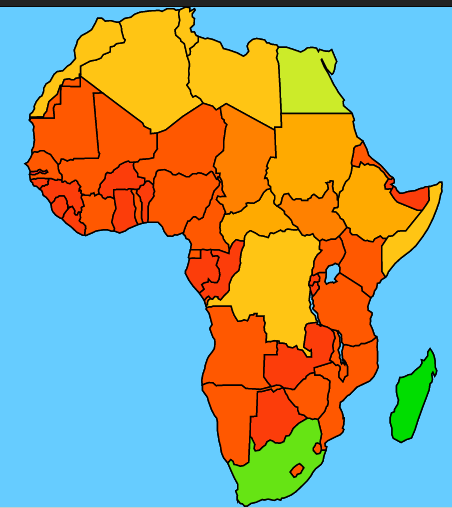
\includegraphics[width=\textwidth]{img/knowledge-map.png}
    \end{column}
  \end{columns}
\end{frame}
% ------------------------------------------------------------------------------
% --------------------------- SLIDE --------------------------------------------
\begin{frame}
	\frametitle{Case Study - Geography facts system}
   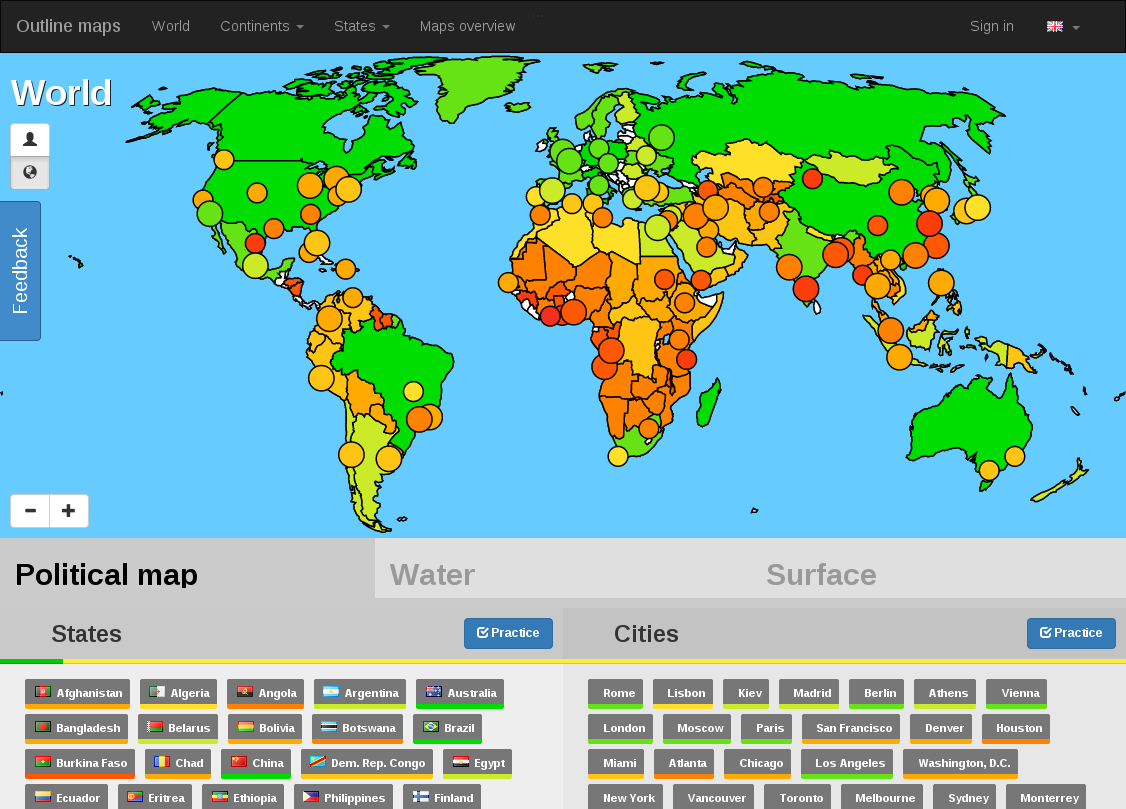
\includegraphics[width=\textwidth]{img/knowledge-map-world-en.png}
\end{frame}
% ------------------------------------------------------------------------------
% --------------------------- SLIDE --------------------------------------------
\begin{frame}
	\frametitle{Practice}
   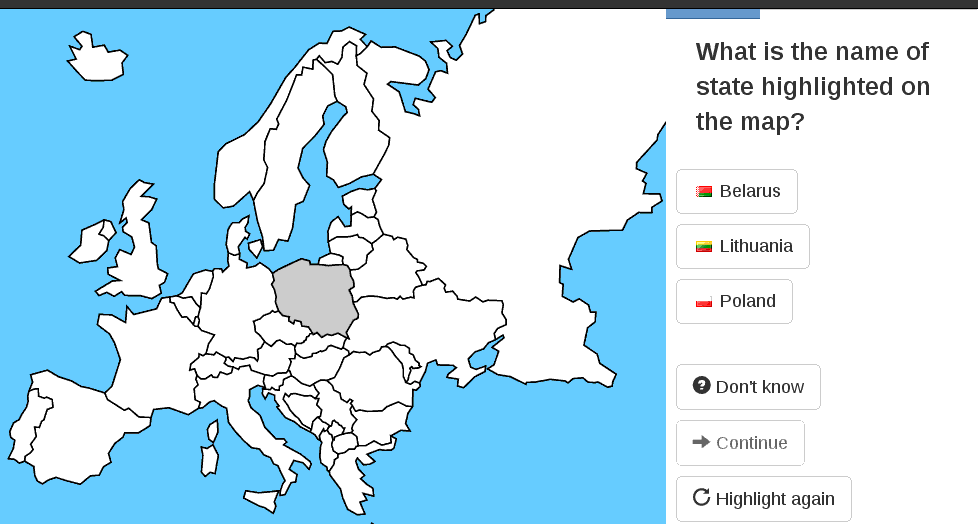
\includegraphics[width=\textwidth]{img/practice-example-en.png}
\end{frame}
% ------------------------------------------------------------------------------
% --------------------------- SLIDE --------------------------------------------
\begin{frame}
	\frametitle{Question Construction Steps}
	 \center{
   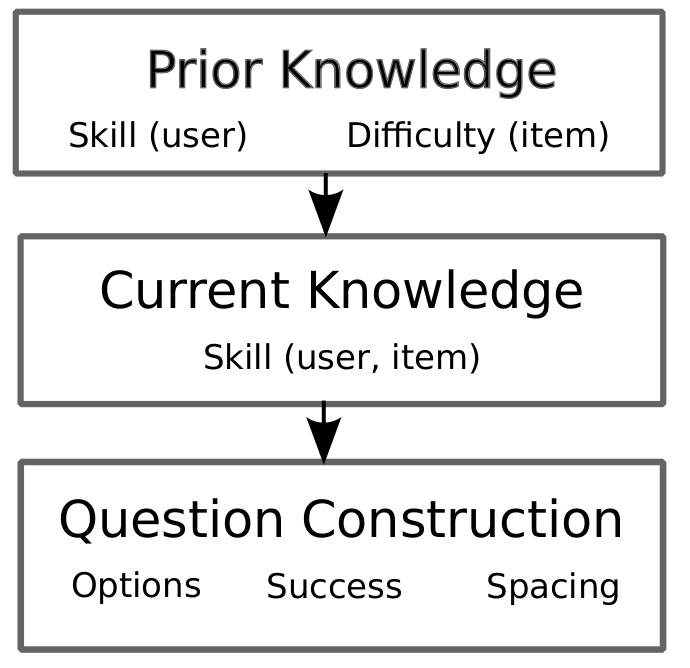
\includegraphics[width=0.5\textwidth]{img/3steps.png}
   }
\end{frame}
% ------------------------------------------------------------------------------
% --------------------------- SLIDE --------------------------------------------
\begin{frame}
	\frametitle{Item Selection – Scoring Functions}
   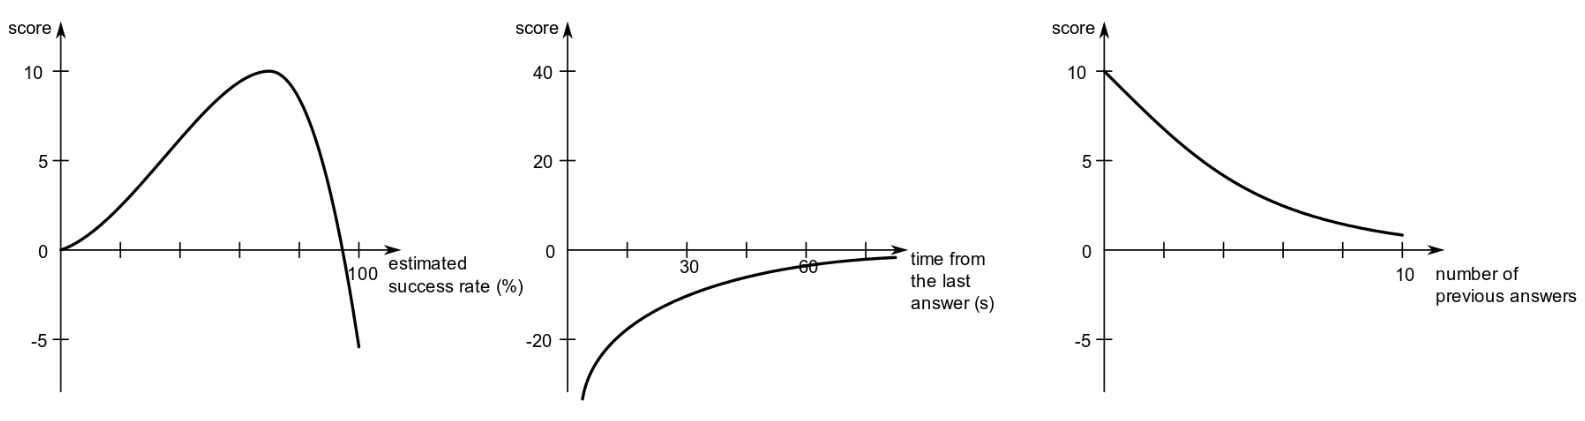
\includegraphics[width=\textwidth]{img/3functions.png}
\end{frame}
% ------------------------------------------------------------------------------
% --------------------------- SLIDE --------------------------------------------
\begin{frame}
  \frametitle{~}
\begin{center} 
\huge{Are adaptive questions better then random?}
\end{center}
\end{frame}
% ------------------------------------------------------------------------------
% --------------------------- SLIDE --------------------------------------------
\begin{frame}
  \frametitle{Are adaptive questions better then random?}
\begin{center} 
\begin{table}[tbh]
  \centering
  \begin{tabular}{lll}
    \toprule
    Condition & Item selection & Options selection \\
    \midrule
    A-A & Adaptive & Adaptive \\
    A-R & Adaptive & Random \\
    R-A & Random & Adaptive \\
    R-R & Random & Random \\
    \bottomrule
  \end{tabular}
\end{table}
\end{center}
\end{frame}
% ------------------------------------------------------------------------------
% --------------------------- SLIDE --------------------------------------------
\begin{frame}
	\frametitle{How to measure it?}
  \begin{itemize}
    \item Success rate increase?
    \item User impression? 
    \item Time in the system? 
    \
  \end{itemize}
\end{frame}
% ------------------------------------------------------------------------------
% --------------------------- SLIDE --------------------------------------------
\begin{frame}
	\frametitle{Results - survivor graph}
   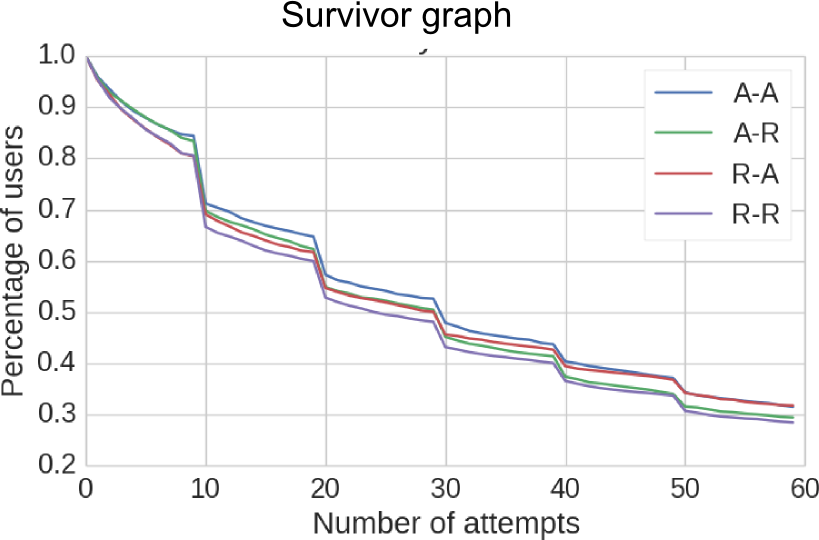
\includegraphics[width=\textwidth]{img/survivor-hack-raw.png}
\end{frame}
% ------------------------------------------------------------------------------
% --------------------------- SLIDE --------------------------------------------
\begin{frame}
	\frametitle{Results - return rate}
\begin{table}
  \centering
  \label{tab:return-prob}
  \begin{tabular}{ll}
    \toprule
    Condition & Return rate \\
    \midrule
    A-A & 	15.1\% \\
    A-R & 	13.9\% \\
    R-A & 	14.3\% \\
    R-R & 	13.1\% \\
    \bottomrule
  \end{tabular}
\end{table}
\end{frame}
% ------------------------------------------------------------------------------
% --------------------------- SLIDE --------------------------------------------
\begin{frame}
	\frametitle{Results - learning curve}
   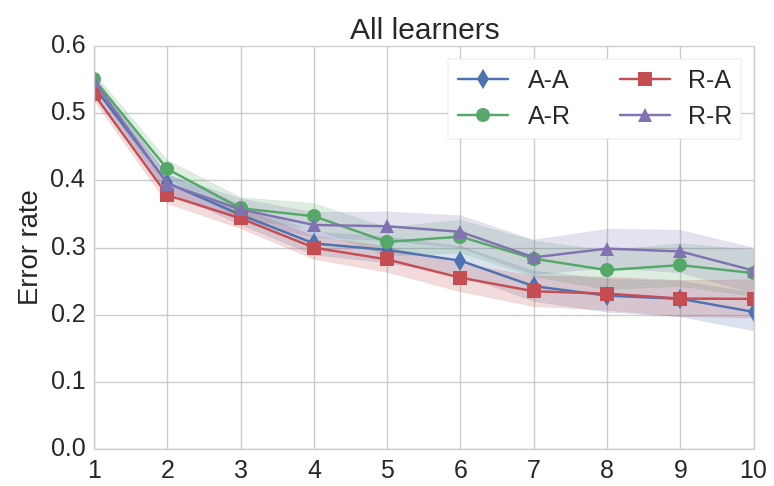
\includegraphics[width=\textwidth]{img/learning_curves_all.png}
\end{frame}
% ------------------------------------------------------------------------------
% --------------------------- SLIDE --------------------------------------------
\begin{frame}
	\frametitle{Results - filtered learning curve}
   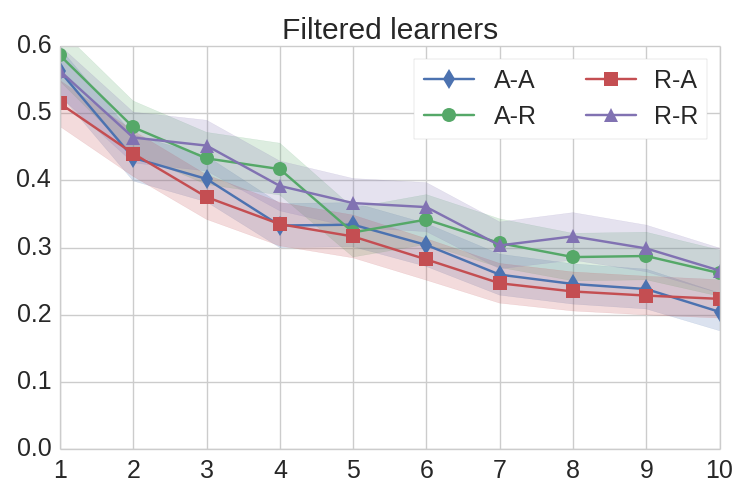
\includegraphics[width=\textwidth]{img/learning_curves_filtered.png}
\end{frame}
% ------------------------------------------------------------------------------
% --------------------------- SLIDE --------------------------------------------
\begin{frame}
	\frametitle{Results - filtered reverse learning curve}
   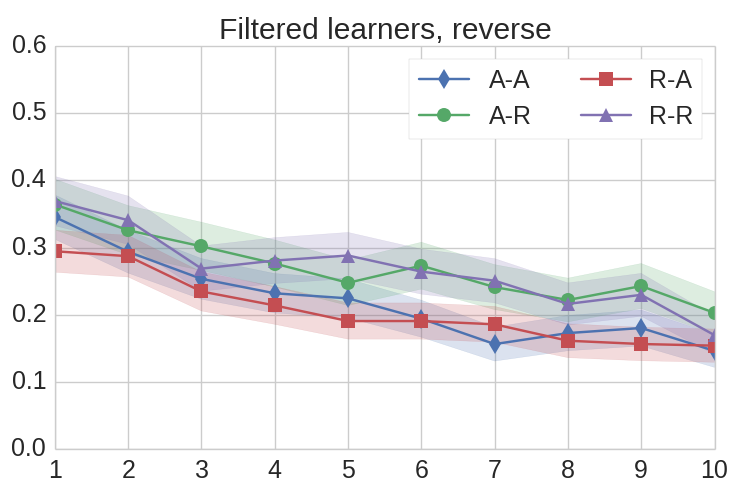
\includegraphics[width=\textwidth]{img/learning_curves_reverse.png}
\end{frame}
% ------------------------------------------------------------------------------
% --------------------------- SLIDE --------------------------------------------
\begin{frame}
	\frametitle{Conclusion}
  \begin{itemize}
    \item Adaptive is better in some aspects
    \item 
    \item 
    \
  \end{itemize}
\end{frame}
% ------------------------------------------------------------------------------
% --------------------------- SLIDE --------------------------------------------
\begin{frame}
  \frametitle{~}
\begin{center} 
\huge  Questions?
\end{center}
\end{frame}
% ------------------------------------------------------------------------------
\end{document}
